\section{System Additions}
Some changes, including a real time kinematic (RTK) global positioning system (GPS) and communication setup, has been added to the system. A full diagram can be seen in \autoref{fig:systemDiagram2}.
%
\begin{figure}[H]
  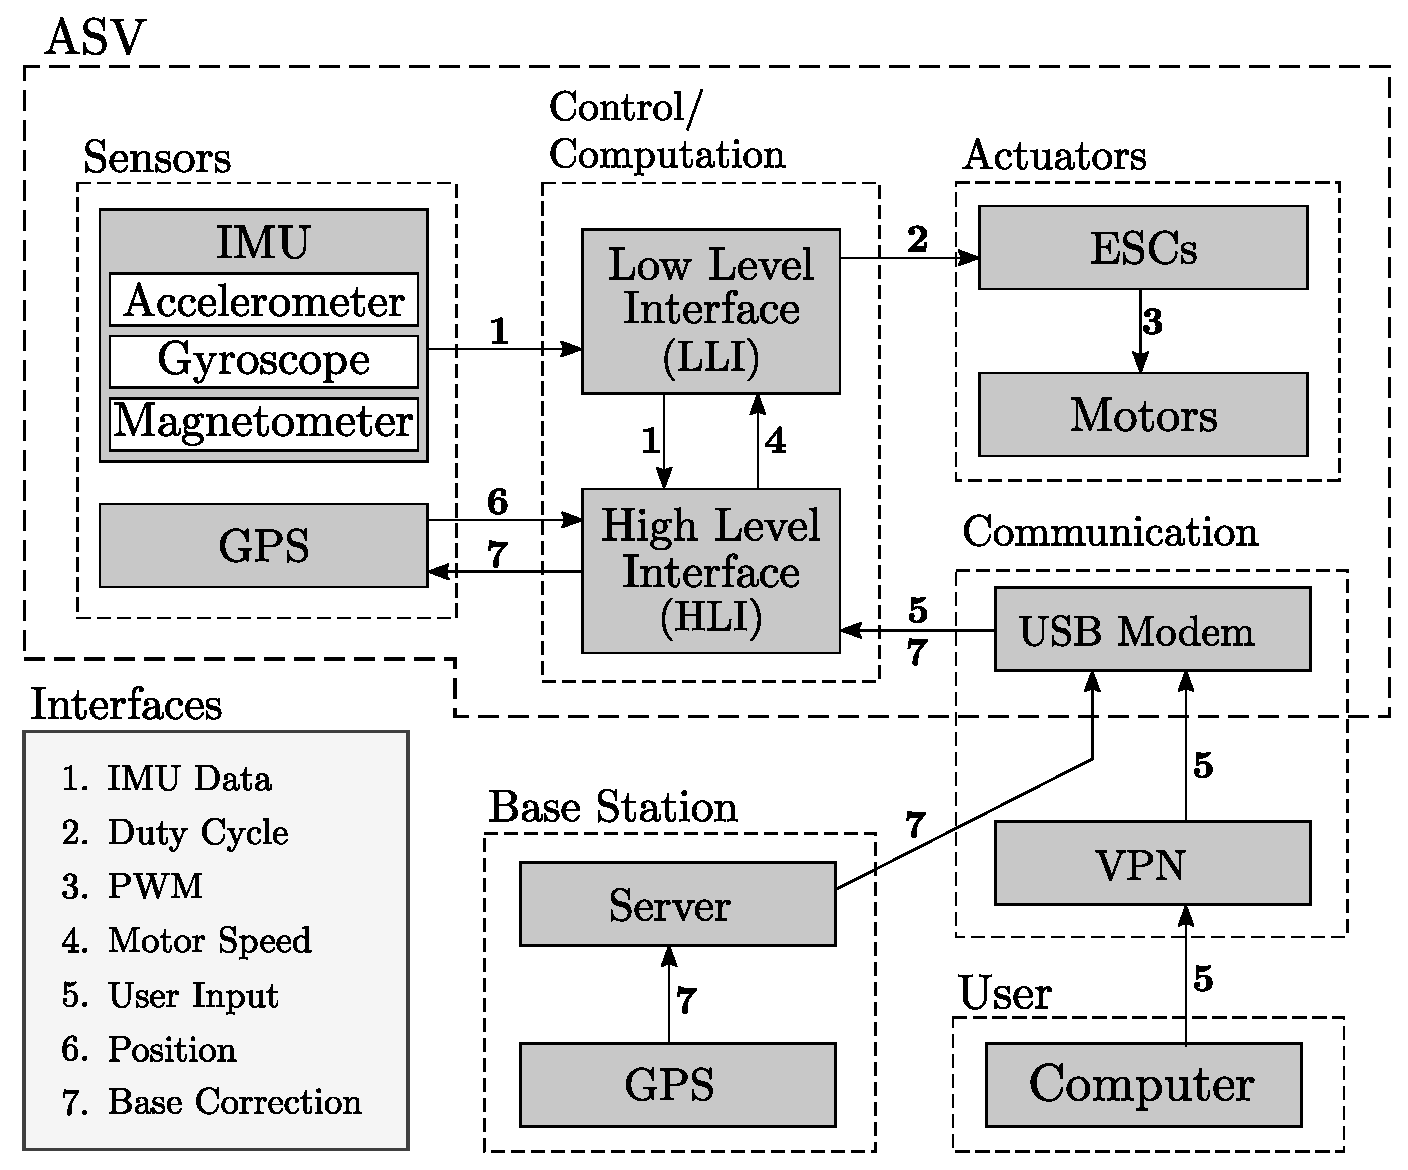
\includegraphics[width=.65\textwidth]{figures/systemDiagram5}
  \caption{A functional diagram of the full system with additions.}
  \label{fig:systemDiagram2}
\end{figure}
%
The RTK GPS system, described in further detail below, is added to obtain better positioning of the ASV. This feature is necessary to accurately map the seabed of the Port of Aalborg with the standards mentioned in \autoref{sec:designconsiderations}.
%This is necessary to obtain sub-meter positioning, without which the control design would have little impact on the performance of the system.\\

Additionally a virtual private network (VPN) server and a USB modem is used to provide user input when the ASV and user are not on the same closed network. This makes it possible to access the ASV through the cellular network and thus eliminates potential problems with regards to range between user and ASV.

\subsection{RTK GPS}
An RTK GPS system consists of two parts, a base station, and a  mobile unit called rover.

The base station is set up at a stationary location with a known, precise GPS position. The rover GPS, mounted on the ASV, measures its location, based on GPS satellites and measurements from the base station. \cite{EmlidRTK}

The modules used in this project, both for the base and the rover, are Emlid Reach RTK GPS, see \autoref{fig:emlidReach}.

\begin{figure}[H]
  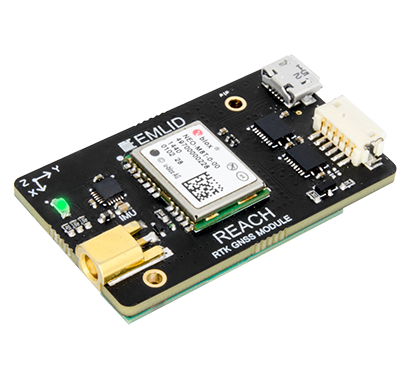
\includegraphics[width=0.27\textwidth]{figures/emlidReach}
  \caption{Emlid Reach RTK GPS module.\cite{EmlidReachDocs}}
  \label{fig:emlidReach}
\end{figure}

The base station gets its current position same as the rover using the same satellites. Since the true position of the base is known, so is the error of each measurement. This is then sent as correction data to the rover, where the error is compensated for. \fxnote{Correct description}

An RTK GPS is able to achieve a higher precision than an ordinary GPS by receiving correction data from a base station, improving from 2-5 m down to a theoretical precision of a few centimeters. \cite{EmlidRTK}

%This data is formatted as an RTCM3 message, which is a protocol designed for this purpose.

\autoref{fig:rtk_GPS} shows how the RTK GPS system is set up. 

\begin{figure}[H]
	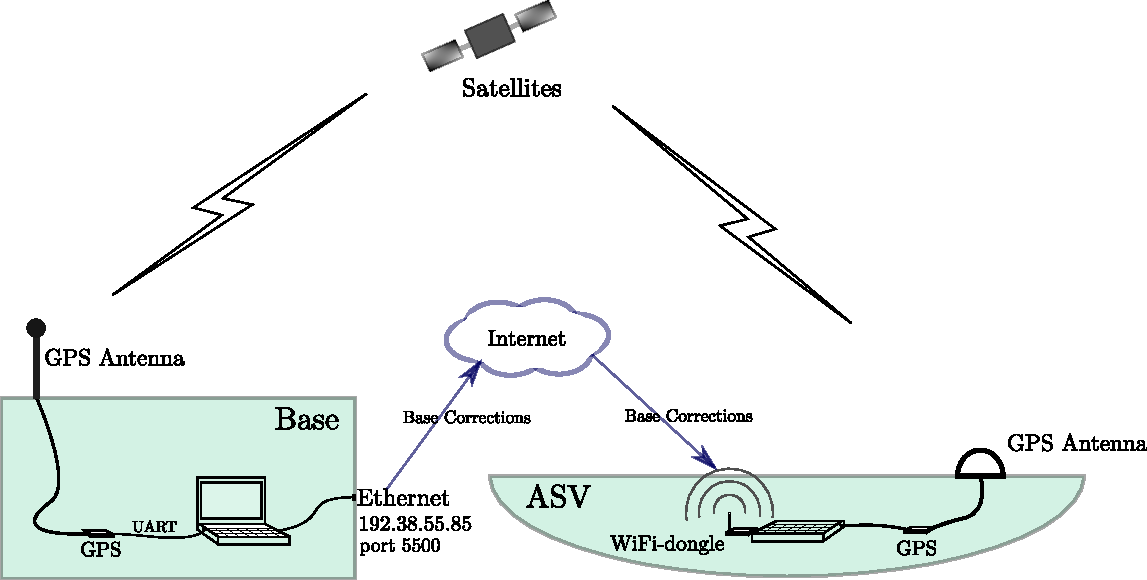
\includegraphics[width=0.8\textwidth]{figures/comunicationSetup.pdf}
	\caption{Overall set up of the GPS.}
	\label{fig:rtk_GPS}
\end{figure}

The base computer forwards the message to a TCP socket, making it accessible through the Internet. The HLI on the vessel connects to this socket and feeds the data to the rover located on the boat. For a more detailed description of the setup see \autoref{app:rtk_gps}.
